\section{Kahden ja kolmen muuttujan funktiot} 
\label{kahden ja kolmen muuttujan funktiot}
\alku
\index{funktio A!c@kahden ja kolmen muuttujan|vahv}
\index{kahden muuttujan funktio|vahv}

\kor{Kahden reaalimuuttujan} funktio on tyyppiä
\[ 
f:\Rkaksi \kohti \R \quad \text{tai} \quad f:A \kohti \R, \quad A\subset\Rkaksi. 
\]
\index{kuvaaja}%
Tällaista funktion \kor{kuvaaja} on Euklidisen avaruuden $\Ekolme$ pistejoukko
\[
G_{f,A}=\{P \vastaa (x,y,z) \in \Rkolme \mid z=f(x,y), \ (x,y)\in A\} \subset \Ekolme,
\]
jonka yleisnimi on \kor{pinta}. Funktiota voidaan 'katsella' esimerkiksi kehittämällä
(yleensä tietokoneen avulla) $G_{f,A}$:n perspektiivikuva. Toinen tapa tehdä kahden muuttujan
funktio geometrisesti havainnolliseksi on piirtää funktion
\index{tasa-arvokäyrä}%
\kor{tasa-arvokäyriä} euklidiseen tasoon. Tasa-arvokäyrä on tason pistejoukko
\[
S_{f,c}=\{P \vastaa (x,y)\in \Rkaksi \mid f(x,y)=c\,\} \subset \Ekaksi \quad (c\in\R).
\]
Kartalla tasa-arvokäyriä ovat \pain{korkeusviivat} ($f=$ maaston 
korkeusfunktio).\footnote[2]{Geometrian käsite \kor{käyrä} on intuitiivisesti ymmärrettynä
'yhtenäinen viiva vailla leveyttä'. Käsitettä on yllättävän vaikea määritellä
täsmällisesti ja samalla yleispätevästi, eikä määrittely edes onnistu pelkin algebran ja 
geometrian keinoin. Sovellustilanteissa kohdataan tyypillisisesti vain käyrien
erikoistapauksia, kuten suoria, toisen asteen käyriä, jne., jolloin käsitteellisiä ongelmia ei
yleensä ole. Tässä ja seuraavissa luvuissa käytetään termiä 'käyrä' intuitiivisesti,
ajatellen lähinnä ongelmattomia erikoistapauksia. --- Termi 'tasa-arvokäyrä' sen sijaan on
sovelluksiakin ajatellen tahallisen huolimaton, sillä kyse voi hyvin olla pistejoukosta, jossa
on 'läiskiä' tai erillisiä pisteitä, tai joukko voi olla tyhjä. Itse asiassa jos $A$ on mikä
tahansa $\Rkaksi$:n osajoukko, niin on helppo määritellä funktio $f$ siten, että $S_{f,c}=A$
annetulla $c$. \index{kzyyrzy@käyrä|av}}
\begin{Exa} \label{saari}
Meren pohjasta kohoavaa saarta kuvaa funktio
\[
h(x,y) = -\frac{1}{10}\,(x^2+2y^2+2xy+4x+14y),
\]
missä $h(x,y)=$ maaston korkeus merenpinnan tasosta (vedenalaisissa osissa $h(x,y)<0$). 
Pituusyksikkö = 100 m. Hahmottele saaren sijainti ja korkeuskäyriä. Missä ja kuinka korkealla 
on saaren korkein kohta?
\end{Exa}
\ratk
Merkitään $\,f(x,y) = -10\,h(x,y)=x^2+2y^2+2xy+4x+14y\,$ ja yritetään ensin kirjoittaa $f$
hieman selkeämpään muotoon
\[
f(x,y)=(x-x_0)^2+2(y-y_0)^2+2(x-x_0)(y-y_0)+c,
\]
eli
\[
f(x,y)=g(\xi,\eta)=\xi^2+2\eta^2+2\xi\eta+c, \quad \begin{cases} \xi=x-x_0,\\ \eta=y-y_0, 
                                                   \end{cases}
\]
missä $x_0,y_0,c\in\R$ on määrättävä. Muunnos $(x,y) \map (\xi,\eta)$ vastaa siis 
koordinaatiston origon siirtoa (toistaiseksi tuntemattomaan) pisteeseen $(x_0,y_0)$.
Vertaamalla $f$:n lausekkeita nähdään, että $x_0,y_0,c$ on valittava siten, että pätee
\begin{align*}
f(x,y) &= x^2+2y^2+2xy-(2x_0+2y_0)x-(2x_0+4y_0)y+(x_0^2+2y_0^2+2x_0y_0+c) \\
       &= x^2+2y^2+2xy+4x+14y \quad \forall (x,y) \in \R^2,
\end{align*}
eli on oltava
\[ \begin{cases} 2x_0+2y_0=-4 \\ 2x_0+4y_0=-14 \\ x_0^2+2y_0^2+2x_0y_0+c=0 \end{cases}
\qekv \begin{cases} x_0=3\\y_0=-5\\c=-29 \end{cases}
\]
Siis $\,\xi=x-3,\ \eta=y+5$, ja
\begin{align*}
f(x,y) = g(\xi,\eta) &= \xi^2+2\eta^2+2\xi\eta-29 \\
                     &=(\xi+\eta)^2+\eta^2-29.
\end{align*}
Viimeksi kirjoitetusta lausekkeesta nähdään, että $g$:n minimikohta $=h$:n maksimikohta on 
pisteessä
\[
(\xi,\eta)=0 \ \ekv \ (x,y)=(3,-5),
\]
ja saaren korkein kohta on 2.9 km meren pinnasta. Saaren rantaviiva on pistejoukko
\[ 
S = \{P \vastaa (x,y) \in \R^2 \mid f(x,y) = 0\}. 
\]
Hahmottelemalla muitakin korkeusviivoja saadaan saaresta yleiskuva. \loppu
\begin{figure}[H]
\begin{center}
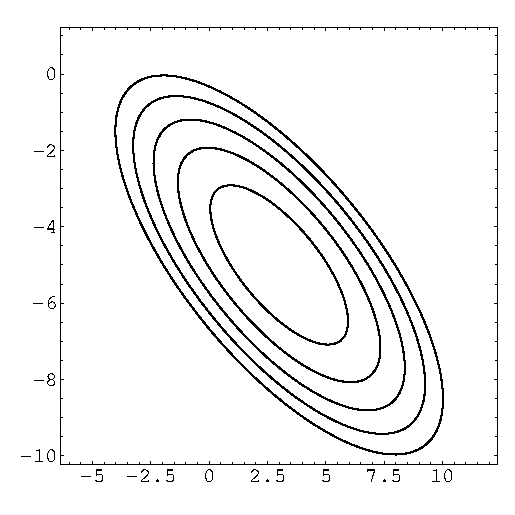
\epsfig{file=kuvat/saari.eps}
\end{center}
\end{figure}
\begin{Exa} Määritä funktion $f(x,y)=x+2y+2$ arvojoukko yksikköneliössä
\[
A=\{(x,y)\in\R^2 \; | \; 0\leq x\leq 1,\; 0\leq y\leq 1\}.
\]
\end{Exa}
\ratk
Tasa-arvokäyrät $S: f(x,y)=c\ $ ovat suoria
%\begin{multicols}{2} \raggedcolumns
\[
x+2y+2=c,
\]
\begin{multicols}{2} \raggedcolumns
joten arvojoukko on (kuva!)
\[
f(A)=[2,5]. \loppu
\]
\begin{figure}[H]
\begin{center}
\import{kuvat/}{kuvaV-1.pstex_t}
\end{center}
\end{figure}
\end{multicols}

\subsection*{Kolmen muuttujan funktiot}
\index{kolmen muuttujan funktio|vahv}

Kolmen reaalimuuttujan funktio on tyyppiä
\[
f:\R^3\kohti\R \quad \text{tai} \quad f:A\kohti\R, \quad A\subset\R^3. 
\]
Kolmen muuttujan funktioita voi havainnollistaa esimerkiksi \pain{vii}p\pain{aloimalla}: 
Valitaan äärellinen joukko muuttujan $z$ arvoja $z_i$ ja tutkitaan kahden muuttujan funktioita
\[
g_i(x,y)=f(x,y,z_i).
\]
\index{zza@\sov!Tomografia}%
\begin{Exa}: \vahv{Tomografia.} \label{tomografia} \ Lääketieteessä paljon käytetyllä 
(tietokone)tomo\-grafialla määritetään nk.\ varjostumafunktio $f$, jonka määrittelyjoukko on
ihmisruumis tai sen osa. Varjostumafunktion arvot ovat reaalilukuja, jotka kertovat
varjostuman tummuusasteen. Funktiosta $f$ saadaan mittausten avulla likimäärin selville
viipaloitujen funktioiden $g_i(x,y)=f(x,y,z_i)$ arvot valituilla (äärellisen monella) $z_i$:n
arvoilla. Funktiot $g_i$ määrätään yhdistämällä suuri joukko erisuuntaisia röntgen(varjo)kuvia 
laskennallisin keinoin (tietokoneen avulla).

Olkoon tarkastelun kohteena (idealisoitu) ihmisen pää
\[
A=\{P \vastaa (x,y,z)\in \R^3 \mid x^2+y^2+z^2\leq 7^2\}
\]
(pituusyksikkö = cm). Tomografiakuvaus tuottakoon varjostumafunktion
\[
f(x,y,z)=1+0.02(2x-3y+6z).
\]
Missä on kirkkainta ja missä tumminta?
\end{Exa}
\ratk Funktio $f$ on saatu käytännössä yhdistelemällä joukko viipalefunktioita
$g_i(x,y)=f(x,y,z_i)$, missä $-7<z_i<7$. Sikäli kuin mittaukset ja niistä lasketut funktiot
$g_i$ ja $f$ katsotaan tarkoiksi, on siis oltava
\[
g_i(x,y)=0.02(2x-3y)+c_i, \quad (x,y) \in A_i\,,
\]
missä $c_i=0.12z_i+1$, ja $A_i$ on kiekon muotoinen leikkauskuvio
\[
A_i=
\{(x,y) \in \R^2 \mid x^2+y^2\leq r_i^2\}, \quad r_i=\sqrt{7^2-z_i^2}.
\]
Funktion $g_i$ tasa-arvokäyrät ovat suoria
\[
2x-3y=\text{vakio},
\]
joten $g_i$:n maksimi ja minimi löytyvät näiden suorien normaalin $3x+2y=0$ ja $A_i$:n 
reunaviivan leikkauspisteistä.
\begin{figure}[H]
\begin{center}
\setlength{\unitlength}{1cm}
\begin{picture}(8,8)(-4,-4)
\put(0,0){\vector(1,0){4}} \put(3.8,-0.4){$x$}
\put(0,0){\vector(0,1){4}} \put(0.2,3.8){$y$}
\put(0,0){\bigcircle{6}}
\multiput(-1,1.5)(1,-1.5){3}{\drawline(-3.5,-2.33)(3.5,2.33)}
\drawline(-2.33,3.5)(2.33,-3.5)
\put(-1.75,2.4){$\bullet$} \put(1.58,-2.6){$\bullet$ $g_i=$max!}
\put(-1.75,3.1){$g_i=$min!}
\put(3,3){$g_i(x,y)=$vakio} \put(2,-4){$3x+2y=0$}
\end{picture}
\end{center}
\end{figure}
Eri viipalekuvia tutkimalla löydetään likimain myös $f$:n maksimi- ja minimiarvot. Tässä
\index{tasa-arvopinta}%
$f$ kuitenkin tunnetaan tarkasti, joten voidaan suoraan tutkia $f$:n \kor{tasa-arvopintoja}.
Nämä ovat tasoja
\[
2x-3y+6z=\text{vakio},
\]
joten voidaan geometrisesti päätellä, että $f$:n maksimi ja minimi löytyvät origon kautta
kulkevan tasa-arvopintojen yhteisen normaalin
\[
\begin{cases} x=2t, \\ y=-3t, \\ z=6t \end{cases}
\]
ja kappaleen reunapinnan
\[
x^2+y^2+z^2=7^2
\]
leikkauspisteistä. Nämä pisteet vastaavat $t$:n arvoja
\[ 
(2t)^2+(-3t)^2+(6t)^2=7^2 \qekv t= \pm 1. 
\]
Varjostuman maksimi- ja minimiarvoiksi päätellään näin muodoin
\begin{alignat*}{3}
&f(2,-3,6)  &\ = 1.98 &= f_{\text{max}}\,, \\
&f(-2,3,-6) &\ = 0.02 &= f_{\text{min}}\,. \qquad\loppu
\end{alignat*}

\subsection*{Funktiot käyräviivaisissa koordinaatistoissa} 
\index{funktio B!h@käyräv.\ koordinaatistoissa|vahv}
\index{muuttujan vaihto (sijoitus)!a@käyräv.\ koordinaatteihin|vahv}
\index{kzyyrzy@käyräviivaiset koordinaatistot!a@--funktiot|vahv}

Kahden ja kolmen reaalimuuttujan funktioita tutkittaessa voi olla apua siirtymisestä 
käyräviivaiseen napa-, lieriö- tai pallokoordinaatistoon silloin kun funktion 
määrittelyjoukon geometria on sellaiseen muunnokseen sopiva. Esimerkiksi, jos kahden
reaalimuuttujan funktio on määritelty pyörähdyssymmetrisessä joukossa $A\subset\Rkaksi$
(voi olla myös $A=\Rkaksi$), voi napakoordinaatteihin siirtyminen auttaa. Siirtyminen tapahtuu
muunnoksella (vrt. Luku \ref{koordinaatistot})
\begin{multicols}{2} \raggedcolumns
\begin{align*}
f(x,y)&=f(r\cos\varphi,r\sin\varphi) \\[2mm]
      &=g(r,\varphi).
\end{align*}
\begin{figure}[H]
\setlength{\unitlength}{1cm}
\begin{center}
\begin{picture}(4,3)(-1,0)
\put(-1,0){\vector(1,0){4}} \put(2.8,-0.4){$x$}
\put(0,0){\vector(0,1){3}} \put(0.2,2.8){$y$}
\put(0,0){\vector(2,3){1.5}}
\arc{1}{5.25}{6.2}
\put(0.5,1.1){$r$} \put(0.5,0.25){$\varphi$} \put(1.45,2.15){$\bullet$ $(x,y)$}
\end{picture}
\end{center}
\end{figure}
\end{multicols}
Huomattakoon, että muunnettu funktio $g$ on itse asiassa yhdistetty funktio
\[
g(r,\varphi)=f(x(r,\varphi),y(r,\varphi)),
\]
missä $x(r,\varphi)=r\cos\varphi,\ y(r,\varphi)=r\sin\varphi$. Siirtyminen 
polaarikoordinaatistosta karteesiseen tapahtuu käänteismuunnoksella
\[
f(x,y)=g(r(x,y),\varphi(x,y)),
\]
missä $\,r(x,y)=\sqrt{x^2+y^2}\,$ ja $\,\varphi(x,y)\,$ on pistettä $(x,y)$ vastaava 
napakulma\footnote[2]{Merkinnöissä $x(r,\varphi)$, $y(r,\varphi)$, $r(x,y)$ ja $\varphi(x,y)$
on alunperin riippumattomista muuttujista $x,y$ tai $r,\varphi$ tehty funktiosymboleja.
Koordinaattimuunnoksissa (myös implisiittifunktioissa, vrt.\ edellinen luku) tällaiset
merkinnät ovat tavallisia, koska ne selkeyttävät laskemista.}
($\varphi$:n laskukaava on hieman konstikas, ks.\ edellisen luvun Esimerkki 
\ref{napakulman kaava}).

Kolmen muuttujan funktioita tarkasteltaessa voidaan siirtyä lieriö- tai 
pallokoordinaatistoon muunnoksilla
\begin{align*}
\text{Lieriö:} \quad  f(x,y,z) &= f(r\cos\varphi,r\sin\varphi,z) =g(r,\varphi,z). \\
\text{Pallo:} \quad\  f(x,y,z) &= f(r\sin\theta\cos\varphi,r\sin\theta\sin\varphi,r\cos\theta)
                                = g(r,\theta,\varphi).
\end{align*}
Lieriökoordinaatiston tapauksessa muunnos $(x,y)\ext(r,\varphi)$, samoin käänteismuunnos
$(r,\varphi)\ext(x,y)$ on sama kuin napakoordinaatistossa. Pallokoordinaatistossa 
käänteismuunnos on
\begin{align*}
g(r,\theta,\varphi) &= g(r(x,y,z),\theta(x,y,z),\varphi(x,y)) \\
&=f(x,y,z),
\end{align*}
missä
\begin{align*}
     r(x,y,z) &= \sqrt{x^2+y^2+z^2}, \\
\theta(x,y,z) &= \Arccos\left(\frac{z}{\sqrt{x^2+y^2+z^2}}\right),
\end{align*}
ja $\varphi(x,y)$ on sama kuin napakoordinaatistossa. Suuntakulma $\theta$ ei ole määritelty
origossa eikä kulma $\varphi$ $z$-akselilla.
\begin{Exa}
Vuoristoisen maaston korkeus merenpinnasta on origon ympäristössä
\[
f(x,y)=x^2-2xy-3y^2+0.2x-0.1y+10
\]
(yksikkö = 100 m). Origossa on kahden tien risteys. Tiet ovat kartalla suoria ja myös niiden
sivuprofiili on suora. Mihin suuntiin tiet kulkevat ja mikä on teiden kaltevuus?
\end{Exa}
\ratk
Siirrytään napakoordinaatistoon:
\[
f(x,y)=h(r,\varphi)=r^2(\cos^2 \varphi-2\cos\varphi\sin\varphi-3\sin^2\varphi) 
                                      + r(0.2\cos\varphi-0.1\sin\varphi) +10.
\]
Tiet noudattavat origosta lähdettäessä puolisuoria $\varphi=\varphi_1$ ja $\varphi=\varphi_2$
(koska ovat kartalla suoria). Koska teiden sivuprofiilikin on suora, on oltava
\[
\cos^2 \varphi-2\cos\varphi\sin\varphi-3\sin^2\varphi=0.
\]
Tässä ei $\,\cos\varphi=0\,$ ole ratkaisu, joten voidaan jakaa $\cos^2\varphi$:lla:
\[
1-2\tan\varphi-3\tan^2\varphi=0 
           \qekv \begin{cases}
                  \,\tan\varphi_1=1/3 \ & \impl \ \ \varphi_1 \approx 18\aste\ 
                                                              \text{tai}\ 198\aste, \\
                  \,\tan\varphi_2=-1 \  & \impl \ \ \varphi_2 =135\aste\
                                                              \text{tai}\ 315\aste.
                  \end{cases}
\]
Kaltevuuskulmat suuntiin $\varphi_1 \approx 18\aste$ ja $\varphi_2=135\aste$ saadaan
ratkaisemalla
\[
\tan\alpha_i=0.2\cos\varphi_i-0.1\sin\varphi_i
                  \qimpl \begin{cases}
                         \,\alpha_1\approx 9\aste, \\
                         \,\alpha_2\approx -12\aste.
                         \end{cases} \qquad\loppu
\]

\begin{Exa}
Etsi (jos mahdollista) pisteet, joissa funktio
\[
f(x,y,z)=xyz(3x^2+3y^2-z^2)/(x^2+y^2)
\]
saavuttaa maksimi- tai minimiarvonsa joukossa
\[
A=\{(x,y,z)\in\R^3 \ | \ x^2+y^2+z^2\leq 96, \ (x,y)\neq (0,0)\}.
\]
\end{Exa}
\ratk Siirrytään pallokoordinaatistoon. Koska pallokoordinaateissa on
\[
x^2+y^2=r^2\sin^2\theta(\cos^2\varphi + \sin^2\varphi)=r^2\sin^2\theta,
\]
niin (vrt.\ Luku \ref{trigonometriset funktiot})
\begin{align*}
f(x,y,z)\,=\,g(r,\theta,\varphi) 
         &=\,r^3\cos\theta\,(3\sin^2\theta-\cos^2\theta)\cos\varphi\sin\varphi \\[2mm]
         &=\,r^3\,(3\cos\theta-4\cos^3\theta)\cos\varphi\sin\varphi \\
         &=-\frac{1}{2}\,r^3\cos 3\theta\sin 2\varphi.
\end{align*}
Funktio $g$ saavuttaa maksimiarvonsa $192\sqrt{6}$ pallon pinnalla $(r=\sqrt{96}=4\sqrt{6})$, 
kun joko $\cos 3\theta=-1$, $\sin 2\varphi=1$ tai $\cos 3\theta=1$, $\sin 2\varphi=-1$. 
Maksimikohtia on neljä:
\[
\begin{array}{llllrr}
(r, & \theta, & \varphi) & (x, & y, & z) \\ \\
(4\sqrt{6}, & \pi/3, & \pi/4) \quad & (\ \: \, 6, &6, &2\sqrt{6}) \\ 
(4\sqrt{6}, & \pi/3, & 5\pi/4) \quad & (-6, &-6, &2\sqrt{6}) \\ 
(4\sqrt{6}, & 2\pi/3, & 3\pi/4) \quad & (-6, & 6, &-2\sqrt{6}) \\ 
(4\sqrt{6}, & 2\pi/3, & 7\pi/4) \quad & (\ \: \, 6, &-6, &-2\sqrt{6})
\end{array}
\]
Minimikohtia (joissa $g=g_{\text{min}}=-192\sqrt{6}$) on samoin neljä. Nämä saadaan vaihtamalla
yhden koordinaatin merkki maksimipisteiden karteesisessa esitysmuodossa. Funktio $g$ saavuttaa
maksimi- tai minimiarvonsa myös pallonpintakoordinaattien arvoilla 
$(\theta,\varphi) \in  \{0,\pi\} \times \{\pi/4,\ 3\pi/4,\ 5\pi/4,\ 7\pi/4\}$. Nämä vastaavat 
kuitenkin karteesisen koordinaatiston pisteitä $(0,0,z)$, jotka ovat alkuperäisen funktion $f$ 
määrittelyjoukon ulkopuolella. \loppu

\subsection*{Usean muuttujan funktioiden yhdistely}
\index{funktio B!e@yhdistetty|vahv}
\index{yhdistetty funktio|vahv}

Useamman reaalimuuttujan reaaliarvoisia funktioita voi yhdistellä yhdistetyiksi funktioiksi 
samoilla periaatteilla kuin yhden muuttujan tapauksessa. Lisäehtona on kuitenkin, että funktiot
ovat tyypiltään yhteensopivia. Esimerkiksi funktioiden $f(x)$ ja $g(x,y)$ yhdistetty funktio 
$F = f \circ g$  voidaan määritellä: 
\[ 
F(x,y) = (f \circ g)(x,y) = f(g(x,y)), \quad \DF_F = \{(x,y) \in \DF_g \mid g(x,y) \in \DF_f\}.
\]
Voidaan myös määritellä yhdistetyt funktiot
\begin{align*}
&G_1(x) = g(x,f(x)),   \quad \DF_{G_1} = \{x \in \DF_f \mid (x,f(x)) \in \DF_g\}, \\
&G_2(y) = g(f(y),y), \,\quad \DF_{G_2} = \{y \in \DF_f \mid (f(y),y)\,\in \DF_g\}, \\
&G_3(x,y) = g(f(x),f(y)),\quad \DF_{G_3} 
                               = \{(x,y) \in \DF_f \times \DF_f \mid (f(x),f(y)) \in \DF_g\}.
\end{align*}
Funktiota $g \circ f$ sen sijaan ei voi määritellä, ei myöskään funktiota $g \circ g$.
\begin{Exa} Jos $f(x) = \sqrt{x},\ \DF_f = [0,\infty)$ ja $g(x,y) = x-y^2,\ \DF_g = \R^2$, niin
\begin{align*}
&F(x,y) = (f \circ g)(x,y) = \sqrt{x-y^2}, \quad \DF_F = \{(x,y) \in \R^2 \mid x \ge y^2\}, \\
&G(x) = g(x,f(x)) = 0, \quad \DF_G = [0,\infty). \loppu
\end{align*} \end{Exa}
\begin{Exa} Määritä funktion $f(x,y) = x^2 + 2y^2 + 2xy + 4x + 14y$ minimiarvo suoralla 
$S:\ y = 2x-5$. (Vrt.\ Esimerkki \ref{saari}.) \end{Exa}
\ratk Kun käytetään suoralla $S$ vallitsevalle funktioriippuvuudelle $x \map y$ 
merkintää $y(x)$, niin kyse on yhdistetystä funktiosta $F(x) = f(x,y(x))$, $\DF_F = \R$.
Koska
\begin{align*}
 F(x) = f(x,2x-5) &= x^2 + 2(2x-5)^2 + 2x(2x-5) + 4x + 14(2x-5) \\[3mm]
                  &= 13x^2 - 18x - 20 \\
                  &= 13\left(x-\dfrac{9}{13}\right)^2 - \dfrac{341}{13}\,,
\end{align*}
niin nähdään, että kysytty minimiarvo on
\[ 
F_{\text{min}} = -\dfrac{341}{13} \approx -26.2. 
\]
Minimikohta on suoran pisteessä $(9/13,-47/13) \approx (0.69,-3.62)$. \loppu

Useamman muuttujan funktioita voidaan yhdistellä myös laskutoimituksin samalla tavoin kuin
yhden muuttujan funktioita (Määritelmä \ref{funktioiden yhdistelysäännöt}).  Ellei
yhdisteltävien funktioiden muuttujien lukumäärä täsmää, on ajateltava, että funktioissa on 
'näkymättömiä' muuttujia. 
\begin{Exa} Jos $f(x) = \tan x\,$ ja $\,g(x,y) = \sin(x+y^2)$, niin kirjoitettaessa
\[ 
F(x,y) = \tan x + \sin (x+y^2) 
\]
tarkoitetaan tämän laskusäännön ilmaisemaa funktiota $F$, määrittelyjoukkona 
\[ 
\DF_F = \{(x,y) \in \R^2 \mid x \neq (n+1/2)\,\pi\,\ \forall n \in \Z\}.
\]
Samaan tulokseen tullaan myös funktioiden yhdistelyn kautta ajattelemalla, että
$F = \tilde{f} + g,\ \DF_F = \DF_{\tilde{f}} \cap \DF_g$, missä $\tilde{f}$ on saatu $f$:stä
lisäämällä toinen muuttuja:
\[ 
\tilde{f}(x,y) = \tan x, \quad \DF_{\tilde{f}} = \DF_f \times \R. \loppu
\] 
\end{Exa}

\subsection*{Kahden muuttujan implisiittifunktiot}
\index{funktio B!j@implisiittifunktio|vahv}
\index{implisiittifunktio|vahv}

Jos $F$ on kolmen muuttujan funktio ja yhtälö
\[
F(x,y,z)=0
\]
ratkeaa $z$:n suhteen, kun $(x,y)\in A\subset\R^2$, niin yhtälö määrittelee $A$:ssa
kahden muuttujan (mahdollisesti monihaaraisen) implisiittifunktion. Jos tälle käytetään
funktiomerkintää $z(x,y)$, niin määritelmä on siis
\[
F(x,y,z(x,y))=0, \quad (x,y)\in A.
\]
\begin{Exa}
Yhtälö $x^2+y^2+z^2=R^2$ määrittelee kaksihaaraisen implisiittifunktion
$z(x,y)=\pm\sqrt{R^2-x^2-y^2}\,$ kiekossa $A:\ x^2+y^2 \le R^2$. \loppu
\end{Exa}
\begin{Exa} Jos $m\in\N,\ m \ge 2$, niin yhtälö
\[
y,z\in\C: \quad y^m=z
\]
määrittelee $m$-haaraisen kompleksifunktion $y=\sqrt[m]{z}$, vrt.\ Luku \ref{III-3}.
Jos kirjoitetaan $z=x+iy$ ja $y=u(x,y)+iv(x,y)$, niin $u$ ja $v$ ovat $m$-haaraisia
funktioita tyyppiä $u,v:\ \Rkaksi\kohti\R$. \loppu
\end{Exa}

\Harj
\begin{enumerate}

\item
Määritä seuraavien funktioiden arvojoukot annetulla janalla $AB$\,: \newline
a) \ $f(x,y)=x^2+2xy-y^2,\,\ A=(1,2),\ B=(-1,3)$ \newline
b) \ $f(x,y,z)=x+xy+yz+z^2,\,\ A=(1,1,1),\ B=(-1,2,-3)$

\item
Määritä seuraavien funktioiden arvojoukot annetussa joukossa $A$: \newline
a) \ $f(x,y)=x+3y-1$, \ $A=$ kolmio, jonka kärjet $(0,1)$, $(4,0)$ ja $(3,4)$ \newline
b) \ $f(x,y,z)=x+2y-3z$, \ $A=\{(x,y,z) \mid (x-1)^2+(y+1)^2+(z-2)^2 \le 9\}$ \newline
c) \ $f(x,y,z)=x+xy+yz+z^2$, \ $A=$ suora $\,2x-2=y+1=4-2z$

\item
Tasangolla $z=0$ on järvi $A=\{(x,y)\in\Rkaksi \mid h(x,y)<0\}$, missä
\[
h(x,y) = 4x^2+y^2+24x+8y
\]
on järven pohjan korkeusprofiili. Tässä $h$ on ilmaistu metreinä ja $x,y$ kilometreinä.
Järven poikki kulkee moottoritie suoraa $y=x+2$ pitkin. Missä on järven syvin kohta ja mikä
on syvyys tässä kohdassa? Hahmottele järven rantaviiva ja laske, missä pisteissä moottoritie
leikkaa rantaviivan.

\item
Muunna seuraavat funktiot napa- tai pallokoordinaatistoon:
\begin{align*}
&\text{a)}\ \ f(x,y)=x+2y \qquad \text{b)}\ \ f(x,y)=xy^2 \qquad 
 \text{c)}\ \ f(x,y)=\frac{xy}{x^2+y^2} \\
&\text{d)}\ \ f(x,y)=\max\{0,x,y\} \qquad
 \text{e)}\ \ f(x,y)=\begin{cases} x^2/y, &\text{kun}\ x > 0\ \text{ja}\ y>0 \\
                                   0,     &\text{muulloin}
                     \end{cases} \\
&\text{f)}\ \ f(x,y)=\begin{cases} xy^2-y^3, &\text{kun}\ 0 \le x \le y \\
                                   0,        &\text{muulloin}
                     \end{cases} \qquad
 \text{g)}\ \ f(x,y,z)=\frac{xyz}{x^2+y^2+z^2} \\
&\text{h)}\ \ f(x,y,z)=\frac{xy^2z^3}{x^2+y^2} \qquad 
 \text{i)}\ \ f(x,y,z)=\begin{cases}
                      \,z^2-xyz, &\text{kun}\ z>0 \\ \,0, &\text{kun}\ z \le 0
                      \end{cases}
\end{align*}

\item
Muunna seuraavat napakoordinaateissa ilmaistut funktiot karteesiseen koordinaatistoon:
\begin{align*}
&\text{a)}\ \ g(r,\varphi)=r^3(\cos\varphi-\sin\varphi) \qquad
 \text{b)}\ \ g(r,\varphi)=\sin 2\varphi-r^2\cos 2\varphi \\
&\text{c)}\ \ g(r,\varphi)=r^2(\tan\varphi+\cot\varphi) \qquad
 \text{c)}\ \ g(r,\varphi)=\frac{\sin\varphi}{2+\cos\varphi}
\end{align*}

\item
Olkoon $f(x,y)=x+y$ ja $g(x,y)=xy,\ (x,y)\in\Rkaksi$. Määrittele sievennettyinä lausekkeina 
(laskusääntöinä) seuraavat yhdistetyt funktiot: \newline
a) \ $f(x,g(x,y))\quad$ b) \ $f(g(x,y),y)\quad$ c) \ $f(g(x,y),g(x,y))$ \newline
d) \ $g(x,f(x,y))\quad$ e) \ $g(f(x,y),y)\quad$ f) \ $g(f(x,y),f(x,y))$ \newline
g) \ $f(f(x,y),f(x,y))\quad$ h) \ $g(g(x,y),g(x,y))$

\item
Olkoon $f(x)=\sqrt{2-x}$ ja $g(x,y)=\sqrt{x-y^2}\ (x,y\in\R)$. Määrittele yhdistetty funktio
$F=f \circ g$ (laskusääntö ja määrittelyjoukko).

\item
Olkoon $f(x)=\sqrt{25-x^2}$ ja $g(x,y)=3x+4y-1\ (x,y\in\R)$. Määritä yhdistetyn funktion
$F=f \circ g$ pienin ja suurin arvo yksikkökiekon neljänneksessä
$A= \{\,(x,y)\in\Rkaksi \mid x \ge 0\,\ja\,y \ge 0\,\ja\,x^2+y^2 \le 1\,\}$.

\item
a) Esitä kompleksifunktion $f(z)=(z+1)^2+(z+i)^2$ reaaliosa, imaginaariosa ja itseisarvo
funktioina tyyppiä $g:\ \Rkaksi \kohti \R$. \vspace{1mm}\newline
b) Määrittele kaksihaaraiset funktiot $u=\{u_1,u_2\}$ ja $v=\{v_1,v_2\}$ siten, että
$u(x,y)+iv(x,y)=\sqrt{z}\ \ \forall z=x+iy\in\C$.

\item
Yhtälö $x+3xyz^2+z^4=0\ (x,y,z\in\R)$ määrittelee implisiittifunktion $z=f(x,y)$. \ a) Laske 
$f$:n arvot pisteissä $(0,0)$, $(2,-1)$ ja $(1,1)$. \ b)  Millaisia ovat $f$:n haarat 
(määrittelyjoukot ja laskusäännöt) yleisemmin?

\item (*)
Vuoristoisen maaston korkeus merenpinnasta on origon $O$ lähellä funktio
\[
f(x,y)=\frac{1}{20}(3x^2-5xy-2y^2)+2.
\]
Origossa on kahden tien $S_1,S_2$ risteys. Tiet ovat maastoon sovitettuja ja vaakasuoria, ja 
lisäksi ne ovat kartallakin suoria. Teiden $S_1,S_2$ poikki kulkee suora rautatie pisteissä
$A\in S_1$, $B\in S_2$. Molemmat pisteet ovat $O$:sta etäisyydellä $1$ (yksikkö = km).
Mikä on suurin pudotuskorkeus laaksoon rautatiesillalta, jonka päät ovat pisteissä $A,B$\,?

\item (*)
Halutaan selvittää, missä pisteissä funktio $f(x,y)=x^2-2xy+3y^2$ saavuttaa suurimman ja 
pienimmän arvonsa\, a) ympyrällä \mbox{$S: x^2+y^2=9$}, \ \ b) kiekossa 
$A=\{(x,y)\in\Rkaksi \mid x^2+y^2 \le 9\}$. Ratkaise ongelma napakoordinaatteja käyttäen 
(vrt.\ Harj.teht.\,\ref{trigonometriset funktiot}:\ref{H-II-5: minmax}).

\item (*)
Funktiosta $f(x)=x-x^3\,$ tiedetään, että välillä $[0,1]$ $f$ saavuttaa suurimman arvonsa
pisteessä $x=1/\sqrt{3}$. Mihin suuntaan origosta lähdettäessä funktio\, a) $f(x,y)=xy^2$,\,
b) $f(x,y,z)=xy^2z^3$ kasvaa nopeimmin suhteessa kuljettuun matkaan?

\item (*) \index{zzb@\nim!Funktio avaimenreiässä} 
(Funktio avaimenreiässä) Olkoon
\[
A=\{\,(x,y,z)\in \R^3 \mid (x,y)\in B_1 \cup B_2,\,\ z\in[0,10]\,\},
\]
missä 
\begin{align*}
B_1 &= \{\,(x,y)\in\Rkaksi \mid x^2+(y-1)^2 \le 2\,\ja\, y \ge 0\,\}, \\
B_2 &= \{\,(x,y)\in\Rkaksi \mid x\in[-1,1]\,\ja\,y\in [-4,0]\,\}.
\end{align*}
Missä $A$:n pisteissä funktio $f(x,y,z)=x-3y+2z$ saavuttaa suurimman ja missä pienimmän arvonsa?

\end{enumerate}

